\section{Numerical methods}\label{app:methods}

\subsection{Runs and checks}\label{app:runs}

The time step is GANDALF's Lawson--Runge--Kutta scheme \citep[Lawson-RK4;][]{Lawson1967}, which integrates the streaming exactly through an integrating factor and treats the nonlinear terms with explicit RK4. Because $A$ does not depend on position, the nonlinear terms $\{\Phi,g\}+s\{\Psi,Ag\}$ of (\ref{mod:hierarchy}) act on the projection of $g$ on each left eigenvector of $A$, with eigenvalue $u_j$, as advection with the stream function $\Phi+su_j\Psi$. An explicit step for them must therefore resolve the speed $\max|\nabla_\perp\Phi|+su_{\max}\max|\nabla_\perp\Psi|$, with $u_{\max}$ the largest eigenvalue of the truncated $A$ (7.25 at $M=32$), not $\max|\nabla_\perp\Phi|+s\max|\nabla_\perp\Psi|$. We take $\Delta t=0.8\times2\sqrt2/\rho$, where $\rho$ is the spectral radius of the advection operator with the stream functions $\Phi\pm su_{\max}\Psi$, computed by a Lanczos iteration every 25 steps, or the Alfv\'enic limit $0.8\,\Delta x/\max|\nabla_\perp z^\pm|$ if that is smaller. The runs at $\beta_i=0.1$ and at $M\ge64$ use a safety factor of 0.4 on the Alfv\'enic limit, with both limits updated every step. The runs at $M=32$ used GANDALF version 0.7.0 on a CPU, and the runs at $M\ge64$ versions 0.8.0 and 0.8.1, whose solver is the same, on a GPU.

The Alfv\'enic turbulence is first spun up with the same forcing and dissipation. Each run then starts from $g=0$, and the averages are over the windows of tables~\ref{tab:runs} and~\ref{tab:mstar}. At $\beta_i=1$, $64^3$ and $M=32$ the run lasts $53\,\tau_A$ and the window is the final $50\,\tau_A$; $W$ reaches its mean level within about $3\,\tau_A$. The window starts at $t=15.5$ in the run at $\beta_i=0.3$ and $M=32$ and at $28.5\,\tau_A$ in the run at $\beta_i=0.3$ and $M=192$, because the free energy was still settling before. At $\beta_i=0.05$ the free energy fluctuates slowly, and those runs are averaged over 160--$300\,\tau_A$.

\begin{table}[t]
  \centering
  \caption{Checks of the run at $\beta_i=1$, $64^3$ and $M=32$ over the window $3\le t\le53$.}
  \label{tab:gates}
  \begin{tabular}{llp{4.4cm}}
    \toprule
    Check & Alfv\'enic & Compressive \\
    \midrule
    Time-stepping error / injected energy & $5.0\times10^{-4}$ & $3.8\times10^{-8}$ \\
    $|\text{injection}-\text{dissipation}|$ / injection & 1.7\% & 0.06\% \\
    Standard deviation / mean of $E_A$ and $W$ & 0.117 & 0.141 \\
    Spread of block means, four blocks of $12.5\,\tau_A$ & 2.4\% ($E_A$) & 8.8\% ($W(m)$), 6.9\% ($\Pi$), 15.5\% ($D_\perp$), 8.4\% ($D_\nu$) \\
    Energy fraction beyond $k_\perp/k_1=21$ & $4\times10^{-5}$ & $2\times10^{-5}$ \\
    Free energy at $m>3M/4$ & -- & 1.1\% \\
    Share of $D_\nu$ at $m\ge M/2$ & -- & 95\% \\
    \bottomrule
  \end{tabular}
\end{table}

\begin{figure}[t]
  \centering
  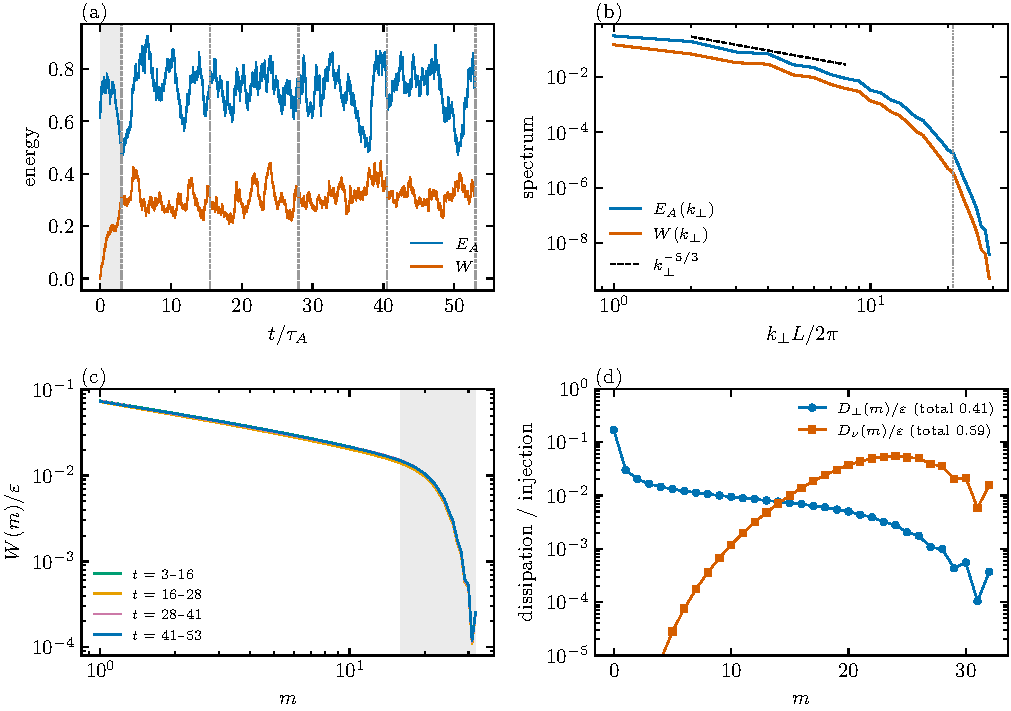
\includegraphics[width=\textwidth]{h1_overview}
  \caption{Overview of the run at $\beta_i=1$, $64^3$, $M=32$. (a) $E_A$ and $W$ against $t$; the dashed lines bound the four averaging blocks, and the shading marks the excluded start. (b) $E_A(k_\perp)$ and $W(k_\perp)$ averaged over $3\le t\le53$, with $k_\perp^{-5/3}$ for reference; the dotted line is the edge of the dealiasing band. (c) $W(m)/\eps$ in each block, divided by the injection rate of that block; the shading marks $m>M/2$, where the hypercollisions act. (d) The rates at which the hyper-resistivity, $D_\perp(m)$, and the hypercollisions, $D_\nu(m)$, remove free energy from moment $m$, as fractions of the injection rate; in total they remove 41\% and 59\% of it.}
  \label{fig:overview}
\end{figure}

\begin{table}[t]
  \centering
  \caption{Fluctuations and convergence of the runs of table~\ref{tab:runs} (upper part, in the same order) and of table~\ref{tab:mstar} (lower part). std/mean is that of $E_A$ and $W$ over the window; the block spread is the largest relative spread of the four block means of $W(m)$, $\Pi$, $D_\perp(m)$ and $D_\nu(m)$; $W_{>}$ is the fraction of the free energy at $m>3M/4$.}
  \label{tab:checks}
  \begin{tabular}{cccccc}
    \toprule
    $\beta_i$ & $N$ & $M$ & std/mean ($E_A$, $W$) & block spread & $W_{>}$ \\
    \midrule
    1 & 64 & 32 & 0.117, 0.141 & 0.155 & 1.1\% \\
    0.3 & 64 & 32 & 0.076, 0.147 & 0.174 & 1.0\% \\
    0.1 & 64 & 32 & 0.120, 0.180 & 0.229 & 0.65\% \\
    1 & 64 & 64 & 0.146, 0.143 & 0.312$^a$ & 1.2\% \\
    0.3 & 64 & 64 & 0.158, 0.136 & 0.185 & 0.87\% \\
    0.1 & 64 & 64 & 0.114, 0.186 & 0.212 & 0.44\% \\
    0.3 & 96 & 64 & 0.133, 0.153 & 0.238$^b$ & 1.02\% \\
    0.3 & 128 & 64 & 0.114, 0.156 & 0.236$^a$ & 1.06\% \\
    0.3 & 256 & 64 & 0.112, 0.123 & 0.162 & 1.19\% \\
    1 & 128 & 64 & 0.112, 0.165 & 0.143 & 1.35\% \\
    1$^c$ & 64 & 64 & 0.156, 0.080 & 0.321$^a$ & 2.15\% \\
    \midrule
    $\beta_i$, $\chi$ & $N$ & $M$ & std/mean ($E_A$, $W$) & block spread & \\
    \midrule
    0.05, 0.96 & 64 & 128 & 0.117, 0.172 & 0.47$^d$ & \\
    0.1, 0.96 & 64 & 64 & 0.114, 0.186 & 0.21 & \\
    0.3, 0.94 & 64 & 192 & 0.124, 0.095 & 0.26$^e$ & \\
    0.05, 0.75 & 64 & 128 & 0.135, 0.139 & 0.18 & \\
    0.05, 0.56 & 64 & 256 & 0.150, 0.143 & 0.12 & \\
    0.05, 0.40 & 64 & 512 & 0.102, 0.107 & 0.16 & \\
    \bottomrule
  \end{tabular}

  \smallskip
  {\footnotesize $^a$ $D_\perp(m)$ at the forced moment: at $m=0$ (31\% and 24\%; 20\% at $m=1$ for $\beta_i=1$), and at $m=1$ in the run with $g_1$ forced (32\%, and 29\% for $W(1)$); at most 19\% for every other average and $m$. $^b$ $W(m)$ at $m=47$ and $D_\nu(m)$ at $m=51$, in the collisional range. $^c$ $g_1$ forced in place of $g_0$. $^d$ $W(m)$ and $D_\nu(m)$ at $m=65$, in the collisional range, from the slow fluctuation of $W$; on the fit range the four block fits of $\ell_*$ agree to within 15\%. $^e$ $D_\perp$ at $m=0$; every other average within 19\%.}
\end{table}

Table~\ref{tab:gates} lists the checks of the run at $\beta_i=1$, $64^3$ and $M=32$, figure~\ref{fig:overview} shows that run, and table~\ref{tab:checks} gives the fluctuations and convergence of every run. Energy is conserved by the time step and balanced between injection and dissipation, in every run to within $2.1\times10^{-3}$ of the injection and to within 2\%. The Alfv\'enic energy fluctuates by 8--16\% about its mean, which at this box size is intrinsic to the forced turbulence. The free energy fluctuates more slowly as $\beta_i$ decreases, so its averages are less certain at low $\beta_i$. We quote the spread of the four block means of each average, each divided by the injection rate of its block, as its uncertainty: at $\beta_i=1$ and $M=32$ the block means agree to within 9\% except $D_\perp$ at $m=0$ (15.5\%), and at $\beta_i=0.1$ the spread is about $\pm12\%$ on $W(m)$. At most 2.2\% of the free energy lies at $m>3M/4$ in any run of table~\ref{tab:runs}, and the spectra show no sign of numerical instability at small scales in any run.

\subsection{Energy accounting}

Each step of the simulations of section~\ref{sec:simulations} consists of GANDALF's Lawson-RK4 step with dissipation and hypercollisions, followed by the forcing increment. The hyper-resistivity and the hypercollisions are linear and diagonal in Fourier and Hermite space, so the free energy they remove from each moment during a step follows from the post-step fields and their damping factors, and the energy before dissipation is reconstructed exactly. The difference between that energy and the energy at the start of the step is the change due to the ideal part of the step, which the exact dynamics conserves; summed over the window it is the time-stepping error of table~\ref{tab:gates}. The injected energy of each step is the change across the forcing increment. This gives $D_\perp(m)$, $D_\nu(m)$ and the injection rate in (\ref{eq:budget}) per moment without finite differences in time, and the field-aligned flux is computed from (\ref{eq:fluxCD}) with GANDALF's dealiased bracket.

\subsection{Field-line tracing}

Field lines of $\bhat=\zhat+\zhat\times\nabla_\perp\Psi$ are integrated in $z$ with the classical fourth-order Runge--Kutta method and step $\Delta z=L/128$ ($L/256$ at $256^3$), with $\nabla_\perp\Psi$ interpolated by cubic B-splines on a grid refined by a factor of two by zero padding. We start 4096 lines at random points of the plane $z=0$ and follow each over four box lengths. Along each line we sample the field of interest and compute its spectrum in the arc length, which equals $z$ to first order in $b_\perp$. The mean field-aligned wavenumber $\kappa_1$ is the first moment of $|\kappa|$ of the spectrum averaged over lines, and we average it over the snapshots of the run. For the injected pattern we draw four fresh realisations of the density forcing with the run's generator and trace them on the same lines; their field-aligned spectrum, averaged over lines, draws and snapshots, is $P(\kappa)$.

\subsection{The frozen copy}\label{app:frozencopy}

To separate structure of $g_0$ along the field from the effect of filtering it in $k_\perp$, we build from each snapshot a field $f$ that equals $g_0$ on the planes $z_n=nL/4$ and, between two neighbouring planes $z_n\le z<z_{n+1}$, is the blend
\begin{equation}
  f(\boldsymbol x_\perp,z)=\cos^2\!\Big(\frac{\pi(z-z_n)}{2a}\Big)\,g_0(\boldsymbol X_n,z_n)+\sin^2\!\Big(\frac{\pi(z-z_n)}{2a}\Big)\,g_0(\boldsymbol X_{n+1},z_{n+1}),\qquad a=\frac L4,
\end{equation}
where $\boldsymbol X_n$ and $\boldsymbol X_{n+1}$ are the points at which the field line through $(\boldsymbol x_\perp,z)$ crosses the two planes, traced as above from every grid point. Along any field line $f$ is a smooth interpolation of the values of $g_0$ at the plane crossings, so it has no field-aligned structure on scales shorter than $a$ apart from that of the blend, while across the field it has the structure of $g_0$; its variance is 83--84\% of that of $g_0$. We trace the same lines as for $g_0$ on the same snapshots, filter $f$, $g_0$ and $\Phi$ into the same bands of $k_\perp$, and compute their spectra along the lines.

\subsection{The two-channel model}

For one field-aligned wavenumber $\kappa$ the model is the forced linear hierarchy
\begin{equation}\label{appD:linear}
  \frac{\dd g}{\dd t}=-\mathsf Lg+\xi\,\boldsymbol e_0,\qquad
  \mathsf L=\ii s\kappa A+\mathrm{diag}\Big(\frac{1}{2T}+\nu\Big(\frac mM\Big)^{n}[m\ge2]\Big),
\end{equation}
where $A$ is the truncated ladder matrix of the run, $\boldsymbol e_0$ the unit vector of $g_0$ and $\xi$ white noise of intensity $q$. The damping $1/(2T)$ of every amplitude removes free energy from every moment at the rate $1/T$. The stationary covariance $\mathsf C=\langle gg^\dagger\rangle$ solves the Lyapunov equation $\mathsf L\mathsf C+\mathsf C\mathsf L^\dagger=q\,\boldsymbol e_0\boldsymbol e_0^{\mathsf T}$. Then $W(m)=p_m\mathsf C_{mm}$, the flux is $\Pi_{m+1/2}=-2s\kappa\,p_mA_{m,m+1}\,\mathrm{Im}\,\mathsf C_{m+1,m}$, and the injection rate is $p_0q$. The model spectrum is the sum of these over the measured $P(\kappa)$, normalised so that the total injection rate equals the measured $\eps$. Free energy injected at $\kappa=0$ does not phase mix and is removed at $m=0$ at the rate $1/T$. At large $m$ and without hypercollisions, the sum reproduces (\ref{eq:Wspread}).

\subsection{Code and data}

The configuration files, the run script and the analysis scripts are in the public repository \url{https://github.com/anjor/krmhd-research}, in the folders \texttt{configs/}, \texttt{scripts/} and \texttt{analysis/} of \texttt{paper/phase-velocity-slices/}; the analysis scripts read only saved data and regenerate every number and figure of section~\ref{sec:simulations} and of this appendix. The self-checking scripts behind sections~\ref{sec:model} and~\ref{sec:frozen} and appendix~\ref{app:branches} are in \texttt{derivations/} of the same folder. The time series, snapshots and analysis outputs of the runs are available from the author on request.
